\chapter{Multirate DSP Algorithms}
\label{chap:multirate}

This chapter explores resampling, and working with a signal path that uses multiple sample rates. Multirate
DSP is not supported by FAUST\autocite{faustwebsite}, and this chapter will cover why this can be very
important in certain classes of DSP algorithms, how the transformations between sample rates is done, and how
I have implemented it in the EDA library. This is all intended as an example of some advantages of working
with a C++ library compared to a DSL.

\section{Aliasing}

According to the Nyquist-Shannon theorem\autocite{shannon49}, a discrete-time sampled signal can only
represent frequencies below half of the sample rate, called the Nyquist frequency $f_N$ or
the Nyquist limit. Intuitively, this is because no change in the waveform can be faster than the time between
two samples.

The frequencies above the Nyquist limit don't just disappear from the sampled signal though, but will instead
be mirrored back and fourth between the Nyquist frequency and $f = 0$. This behaviour is
called aliasing, and is undesirable in most usecases, since it distorts the signal with non-harmonic
frequencies.

When initially sampling an analog signal, the main way to avoid aliasing is simply to use an analogue
low-pass filter to remove any frequencies above the Nyquist limit before the signal is sampled to discrete
time\autocite{an699},  which means there are no frequencies to be aliased. However, aliasing can also
be an issue in some DSP operations that introduce new frequencies above the original signal, such as
nonlinear waveshaping functions, i.e. an operation that applies a function $\omega(x)$ to the
original signal $x$, where $\omega$ is non-linear.

\begin{figure}
  \centering
  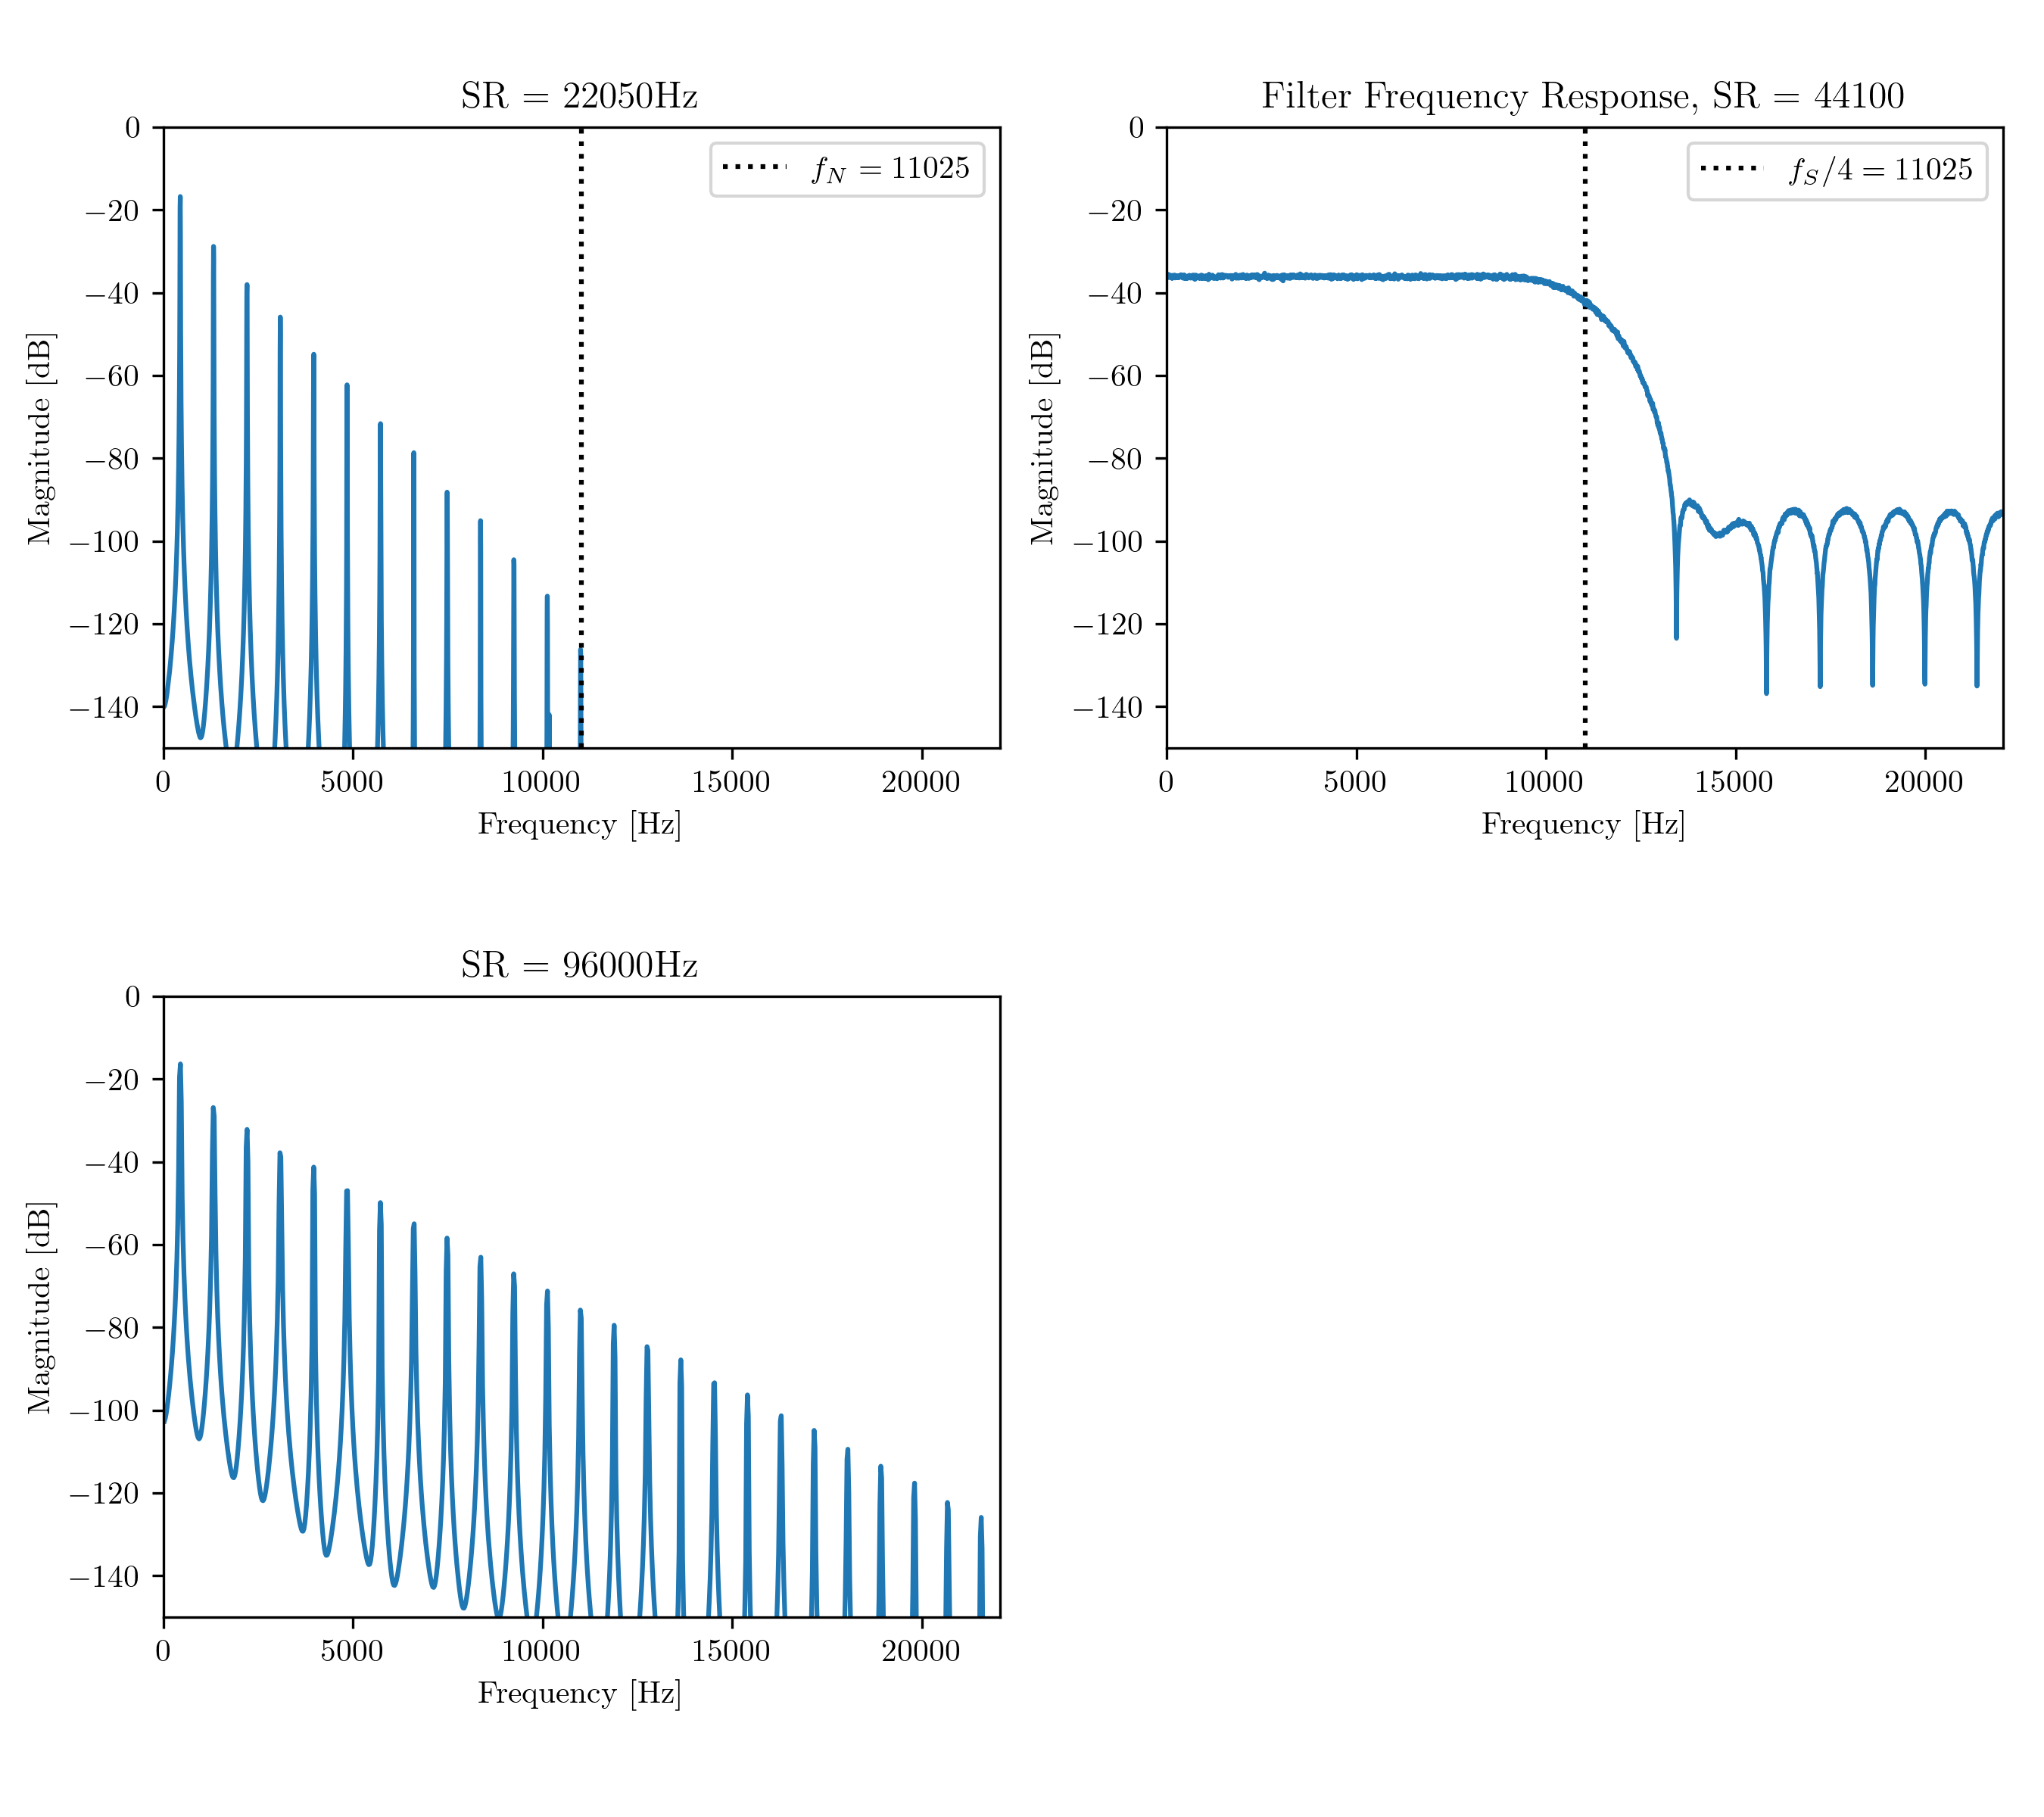
\includegraphics[width=\textwidth]{Pictures/resampled_tanh.png}
  \caption{
    A \SI{1800}{Hz} sine wave passed through the nonlinear waveshaping function $\omega(x) = \tanh(5x)$ at
    different sample rates and resampling factors $N$. Given the high
    samplerate, (a) can be seen as representing the
    ideal signal over this frequency range. (c) and (d) additionally show the frequency response of the
    interpolation/decemation filters used with oversampling. For better visualization, the logarithmic decibel  scale is used on the vertical axis: $ z\; \mathrm{dB} = 20 \cdot \log_{10}(z) $.
  }
  \label{fig:resampled_tanh}
\end{figure}

\subsection{Waveshaping Distortion}

A simple and common example of nonlinear waveshaping is distortion using the hyperbolic-tangent trigonometric
function $\omega(x) = \tanh(x)$ (or, in practice, a polynomial approximation thereof). By adjusting the gain
of the input, i.e $\omega(x) = \tanh(g\cdot x)$, the effect can span from a soft saturation to hard clipping. When
looking at the frequency spectrum, this introduces frequencies above the original signal, and in the case
where the input is a simple sine wave (i.e. a single peak frequency), this waveshaping operation introduces
odd harmonics, that is it introduces frequencies at odd multiples of the frequencies in the original signal.
Adjusting the gain will change the magnitude (volume) of these frequencies.

In the following introduction to aliasing and oversampling, I will refer heavilly to the graphs in
\autoref{fig:resampled_tanh}. These are visualizations of various runs of this waveshaping distortion, all with an
input signal of a sine wave at \SI{1800}{Hz}, and $g = 5$. These parameters were
chosen simply because of the visualizations they result in, but do reflect real-world usecases. (a) is
generated at a very high sample rate relative to the visible frequency range, and can be regarded as
representing the ideal signal. Here, the fundamental frequency at \SI{1800}{Hz} is visible as the
first peak, and the harmonics can be seen at even intervals above the fundamental.

\autoref{fig:resampled_tanh} (b) shows the same signal operation applied at 22050Hz, where the aliasing becomes
evident. Notice that the added frequencies are a clear mirroring back and forth between the Nyquist frequency
and 0 Hz. It should be very clear that these frequencies are unwanted, and it is especially worth noting that
the aliasing has added frequencies below the fundamental, which will be particularly noticable. The signal we
actually want when applying $\omega$ at 22050Hz, is the left half of (a), i.e. all the
frequencies of the ideal signal that are representable at that sample rate, i.e. the ones that are below the
Nyquist limit of 11025Hz.

\section{Oversampling for Alias reduction}
The most common approach to reduce the effects of aliasing in DSP algorithms, is oversampling, which is the
operation of upsampling by a factor of $N$, performing the required operations on the
signal, and then downsampling by $N$ again, to return to the original sample rate. The
basic idea is, that by raising the sample rate, you raise the Nyquist frequency, which means the point at
which frequencies will be mirrored is raised. This results in a smaller part of the signal being mirrored,
and the first area that the loudest frequencies will be mirrored onto, is above the original Nyquist limit,
and can be removed when downsampling to the original sample rate.

The effects of this process can be seen in \autoref{fig:resampled_tanh}, where (c) and (d) show the operation
applied with upsampling of $N = 2$ and $N = 4$. Ignoring the frequency response
of the filter (shown in orange), these plots clearly show less aliasing, with no visible aliasing at all for
$N = 4$. With $N = 2$ it can be seen that the mirroring has happened at
$f = \SI{22050}{Hz}$ instead, but then the frequencies above $\SI{11025}{Hz}$ have been filtered out.
This clearly shows how oversampling reduces the effects of aliasing, and for this operation with this data,
it looks like $N = 4$ is enough. However, $N = 8$ is often chosen in the more
general case \autocite{kahles2019oversampling}

There are other and more efficient ways to avoid aliasing\autocite{7865908}, but they mostly depend on
specific knowledge of the nonlinear operation that is being used, and oversampling is widely recognized as
the standard method for alias reduction\autocite{kahles2019oversampling, deman2014}.

\subsection{Interpolation}
\label{sec:interpolation}

I will briefly introduce the most common method of increasing the sample rate of a sampled signal, in which
the signal is first zero-stuffed and then interpolated using a filter. Like with alias reduction, this is an
area where many variants and other methods have been developed\autocite{SORIA2013, castillocomparative}, and this section vastly
simplifies the subject. However, it gives a general understanding of the problems involved, and how they are
most commonly solved.

It is also worth noting that the terms \emph{upsampling} and \emph{interpolation} are often conflated.
This can lead to some confusion, however when not talking about the implementation details of either, both
terms usually refer to the joint operation of upsampling and interpolation.

The first step is to simply increase the sample rate of the signal. This is done by \emph{zero-stuffing}
the signal, i.e. inserting $N - 1$ zeros between each sample. In \autoref{fig:interpolation} the
result of this operation can be seen in the time and frequency domains. In the frequency domain, two things
have happened: The gain of the signal has been scaled by $\frac{1}{N}$, and the signal has been
mirrored around the old Nyquist frequency $f_{N1}$. The gain is simply restored by multiplying
each sample by $N$, and for the new signal above $f_{N1}$, we can use a low
pass filter to remove them.

\begin{figure}
  \centering
  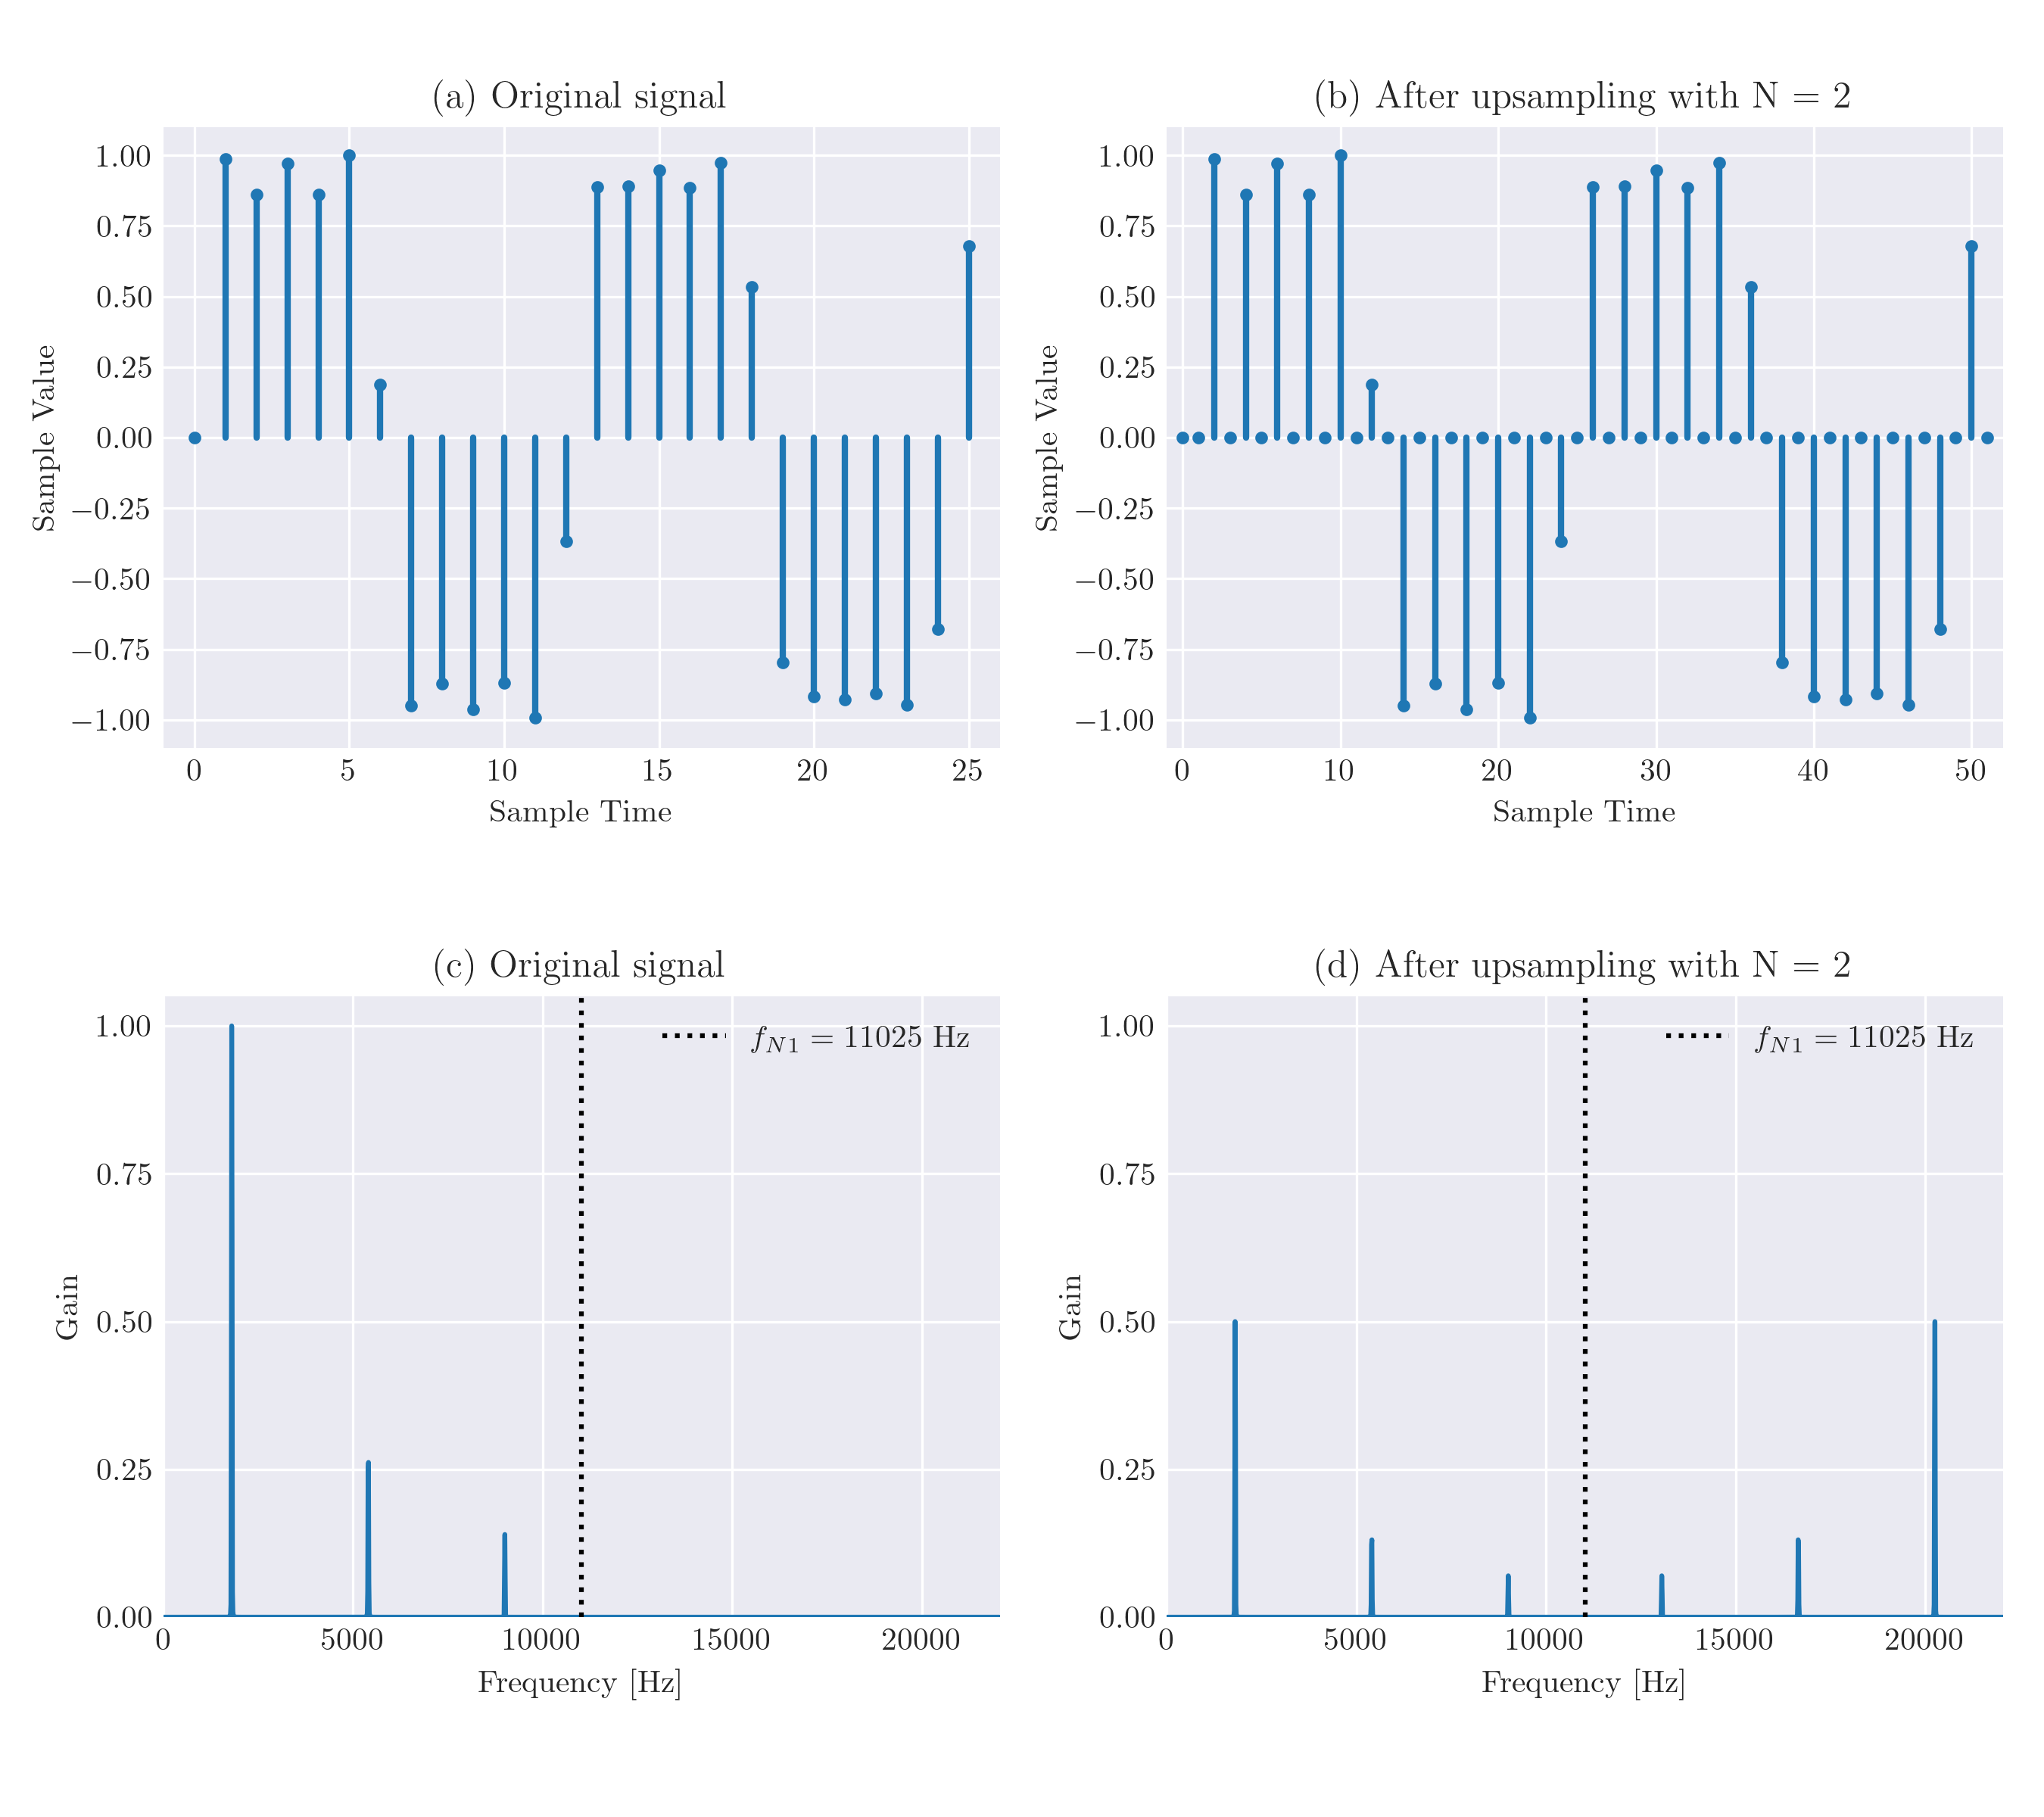
\includegraphics[width=\textwidth]{Pictures/interpolation.png}
  \caption{The effects of zero-stuffing on the waveform and frequency spectrum. The input signal is the same saturated
    1800Hz sine wave as used in \autoref{fig:resampled_tanh}, and the sample rates are 22050Hz and 44100Hz before and  after upsampling respectively. To clearly show the
    reduction in gain on upsampling, linear gain is used on the vertical axis of the frequency graphs.}
  \label{fig:interpolation}
\end{figure}

\subsection{FIR Filters}
\label{sec:fir_filters}

There are a lot of methods to designing and implementing interpolation filters for the best and most
efficient results, but most of them are based on Finite Impulse Response (FIR) filters. A FIR filter of order
$N$ is a simple convolution operation where each output is a weighted sum of the
$N + 1$ most recent inputs. Designing FIR filters, i.e. picking the right coefficients, is a
heavilly researched topic\autocite{kahles2019oversampling, SORIA2013, thomas2009}, and not something I will go into in this project, however,
the filters used for testing and for \autoref{fig:resampled_tanh}, are FIR filters of order $N = 128$,
designed using the method described in \autocite{fiir}. These filters have a fairly high order to
ensure a very steep cutoff, but in real use there is a tradeoff between the efficiency of a lower filter
order, and the better results of a harder cutoff point.

\subsection{Decimation}
\label{sec:decimation}

When downsampling, we first need to remove any frequencies above the Nyquist limit of the resulting sample
rate, since those will otherwise be aliased, which was the original reason for oversampling. This process is
called \emph{decimation}, and consists of running a lowpass filter and then selecting every
$N^\mathrm{th}$ sample for output. Thus, it closely resembles interpolation, and in fact the same
filter can be used for both, even though different ones are often used for the best results, partly because
decimation allows for some special optimizations, as only every $N^\mathrm{th}$ sample is actually
required, which means some computations can be skipped in the FIR filter. These topics are covered in many of
the referenced sources of this chapter, such as \autocite{kahles2019oversampling, SORIA2013, thomas2009}.

\section{Multirate in the Algebra of Blocks}
\label{sec:multirate_blocks}

Now that we know why resampling is important, and the basics of how it is implemented, I will look at how to
integrate it in the block algebra introduced in \autoref{chap:blocks}.

\subsection{Approach I}
\label{sec:multirate_blocks_1}
In the most general model, multirate blocks are introduced by adding an extra parameter
$R$ to signals, as the ratio of the sample rates $f_{out}/f_{in}$. This means blocks
will be defined with the types $i \rightarrow_R o$, and block compositions need type rules to compute the
rate ratio as well. As an example, here is the type rule as it would be stated for \Sequential:

\begin{prooftree}
  \AxiomC{$d_1 : n \rightarrow_{r} p$}
  \AxiomC{$d_2 : p \rightarrow_{q} m$}
  \BinaryInfC{$\Sequential(d_1, d_2) : i_1 \rightarrow_{r \cdot q} o_2$}
\end{prooftree}

This means the rate ratio of $\Sequential(d_1, d_2)$ is the product of the rate ratios of
$d_1$ and $d_2$. Similarly, $\Parallel(d_1, d_2)$ requires both operands
to have the same rate ratio, which becomes the rate ratio of the compositio n. One would then introduce
$\Block{upsample}(n) : 1 \rightarrow_n 1$ and $\Block{downsample} : 1 \rightarrow_{\frac 1
    n} 1$ blocks, which could be used to change the sample rate.

This model has the advantage of allowing other uses for resampling, such as interfacing between two systems
that use different sample rates, as a top-level signal processor can have different input/output sample
rates. However, it introduces a large amount of complexity to evaluating the signal processors, since blocks
that downsample can only output after receiving $\frac 1 R$ samples, and blocks that upsample
output $R$ samples at a time.

\subsection{Approach II}
\label{sec:multirate_blocks_2}

Instead, a simpler approach is chosen, where all blocks have the same input/output rate, but a separate
$\Resample\left<N\right>(d, F_i, F_d)$ block is introduced, which can be used to perform oversampling for the block
$d$, with ratio $N$, interpolation filter $F_i$, and
decimation filter $F_d$. This means, that while $d$ is evaluated at a
higher sample rate, the full $\Resample$ block outputs at the same sample rate as its input. This
block can be seen in \autoref{fig:block_resample}, and the type rules and signal processesor of it are described
here:

\begin{prooftree}
  \AxiomC{$d : i \rightarrow o$}
  \AxiomC{$F_i : i \rightarrow i$}
  \AxiomC{$F_d : o \rightarrow o$}
  \AxiomC{$N \in \mathbb{N}^+$}
  \QuaternaryInfC{$\Resample\langle N\rangle(d, F_i, F_d) : i \rightarrow o$}
\end{prooftree}

\begin{prooftree}
  \AxiomC{$\begin{array}{l}
        u_j(t) = \begin{cases}
          s_j\left(\frac t N\right) & \exists k \in \mathbb N : t = N \cdot k \\
          0                         & \textrm{otherwise}
        \end{cases}                                                \\
        \SigP{\Sequential(\Sequential(F_i, d), F_d)}(u_1, \dots, u_i) = (v_1, \dots, v_o) \\
        y_j(t) = v_j(t \cdot N)
      \end{array}$}
  \UnaryInfC{$\SigP{\Resample\langle N\rangle(d, F_i, F_d)}(s_1, \dots, s_i) = (y_1, \dots, y_o)$}
\end{prooftree}

\begin{figure}
  \centering
  \includestandalone[]{Pictures/block_resample}
  \caption{The resample block as implemented in the EDA library}
  \label{fig:block_resample}
\end{figure}

While this approach does not allow a signal processor to output at a different rate than its input, it still
covers most relevant usecases. For instance, all plugin frameworks mentioned in the previous chapter have
this constraint. In general, actual sample-rate conversion is usually done at the edge of the system, and in
the cases where it is needed, it can easily be done outside of the component described as a block diagram.

\section{Multirate in the EDA Library}
\label{sec:multirate_eda}

As with most of the constructs described in \autoref{chap:cpp_lib}, translating the resampling block to C++
for the EDA library is a fairly straight forward process. \Resample is a compositional block, so it inherits
from \cpp{CompositionBase}. In the implementation shown here, the filters are just sequentially composed
around the inner block in the construction function, but in an optimized implementation custom filters would
be used, with optimizations such as not invoking the decimation filter on the samples that are discarded
during downsampling (see \autoref{sec:decimation}).

\begin{cppcodenl}
  template<int N, AnyBlock Block>
  requires(N > 1)
  struct Resample : CompositionBase<Resample<N, Block>, ins<Block>, outs<Block>, Block> {};

  template<int N>
  constexpr auto resample(AnyBlock auto block, AnyBlock auto f1, AnyBlock auto f2)
  {
    auto filter_block = seq(f1, block, f2);
    return Resample<N, decltype(filter_block)>{{filter_block}};
  }
\end{cppcodenl}

The evaluator is where the interesting parts recide:

\begin{cppcode}
  template<int N, AnyBlock Block>
  struct evaluator<Resample<N, Block>> : EvaluatorBase<Resample<N, Block>> {
    constexpr evaluator(const Resample<N, Block>& resample) noexcept
    : EvaluatorBase<Resample<N, Block>>(resample)
    {}

    constexpr Frame<outs<Block>> eval(Frame<ins<Block>> in)
    {
      auto& e = std::get<0>(this->operands);
      for (float& f : in) {
        f *= N;
      }
      Frame<outs<Block>> res = e.eval(in);
      for (int i = 1; i < N; i++) {
        e.eval({});
      }
      return res; 
    }
  };
\end{cppcode}

\begin{itemize}
  \item \textit{Line 10-12}: The gain is increased to compensate for the loss during interpolation (see
        \autoref{sec:interpolation})
  \item \textit{Line 13}: The block is evaluated on the input data.
  \item \textit{Line 14-16}: The block is evaluated $N - 1$ times with all-zero inputs.
  \item \textit{Line 17}: The result of the first evaluation is returned.
\end{itemize}

Since the block here already contains the interpolation/decimation filters, these operations constitute
oversampling.

\subsection{FIR filters in EDA}

While Finite Impulse Response filters (as introduced in \autoref{sec:fir_filters}) are used for many other
purposes than rate conversions, the implementation is included in this chapter for context.  Given filter
kernel $(b_0, b_n)$, the block $\Block{fir}(b_0, \dots, b_n) : 1 \rightarrow 1$ is a primitive block implemented as such:

\begin{cppcodenl}
  template<std::size_t N>
  struct FIRFilter : BlockBase<FIRFilter<N>, 1, 1> {
    std::array<float, N> kernel;
  };

  template<std::size_t N>
  constexpr auto fir(std::array<float, N> kernel) noexcept
  {
    return FIRFilter<N>{.kernel = kernel};
  }
\end{cppcodenl}

I will not go into detail on the implementation, but it is shown here mainly to illustrate that except for
the EDA-speciffic structure of the classes, the filter is implemented in normal C++, similar to how a
point-wise evaluated FIR filter would usually be implemented, with a \cpp{std::array} used as a
ringbuffer, the kernel stored in two consecutive copies, and the meat of the evaluation being done with
\cpp{std::inner_product}\footnote{see \url{https://en.cppreference.com/w/cpp/algorithm/inner_product}}:

\begin{cppcodenl}
  template<std::size_t N>
  struct evaluator<FIRFilter<N>> : EvaluatorBase<FIRFilter<N>> {
    constexpr evaluator(const FIRFilter<N>& fir) noexcept
    {
      std::ranges::copy(fir.kernel, kernel.begin());
      std::ranges::copy(fir.kernel, kernel.begin() + N);
    }
    constexpr Frame<1> eval(Frame<1> in)
    {
      if (t == N) t = 0;
      t++;
      z[N - t] = in;
      auto start = kernel.begin() + t;
      return std::inner_product(start, start + N, z.begin(), 0.f);
    }
    private:
    std::size_t t = 0;
    std::array<float, N> z = {0};
    std::array<float, 2 * N> kernel;
  };
\end{cppcodenl}

This implementation shows that it is possible to implement DSP algorithms in "normal" C++, which allows for
hand-written optimizations and complex state, and still have them completely transparently available as a
block in an EDA context.

\subsection{Example}

To demonstrate oversampling in EDA, the $\tanh(5x)$ example used throughout this chapter is
implemented in EDA as such:

\begin{cppcodenl}
  auto quarterpass = fir(qp_coefficients);
  auto tanh = fun<1, 1>(&std::ftanh);
  auto saturation = resample<4>(_ * 5 | tanh, quarterpass, quarterpass);
\end{cppcodenl}

In fact, LV2 plugins constructed in a manner similar to the echo plugin described in \autoref{sec:echo_plugin}
containing variations on this implementation is what was used to generate \autoref{fig:interpolation} and
\autoref{fig:resampled_tanh}.

The coefficients for the filter can be seen in the appendix, page \pageref{codefile:include/eda/resampling.hpp}.

\section{Conclusion}

This chapter has covered the motivation and methods behind multirate DSP, with a focus on oversampling. By
implementing this feature in the algebra of blocks, and then in the EDA library in roughly 30 lines of code,
I have given an example of the merits of a domain specific library in a general-purpose language compared to
a domain specific language, and specifically the versatility allowed by the design choices made in this
project. To help support this argument, an implementation of a FIR filter was shown, illustrating how
complicated primitive blocks can be implemented in vanilla C++ by the user of the library, instead of having
to rewrite the problem in terms of recursion and other basic compositional blocks.

In \autoref{sec:multirate_blocks}, two possible solutions for multirate DSP were introduced, and while the second
was selected here, the first also has potential, though the implementation would be more involved. It does
however enable operations that are not supported by the chosen design, by allowing blocks to output at a
different sample rate than their input. Potential further work in this area includes exploring possible
implementations of that design, and especially how it would integrate with work on vectorization and
buffer-wise evaluation.
